\section{Planificación, metodología y presupuesto}

En esta sección, se van a definir los componentes fundamentales en la gestión del proyecto. Estos permitirán definir claramente los objetivos, los recursos disponibles y cómo se utilizarán para alcanzar los resultados deseados dentro de un marco de tiempo y costos preestablecidos.

\subsection{Planificación temporal}

Se ha elaborado un calendario, marcando con colores los plazos (en días) de las distintas tareas y subtareas en las que se ha desglosado el proyecto.

\begin{figure}[H]
	\centering
	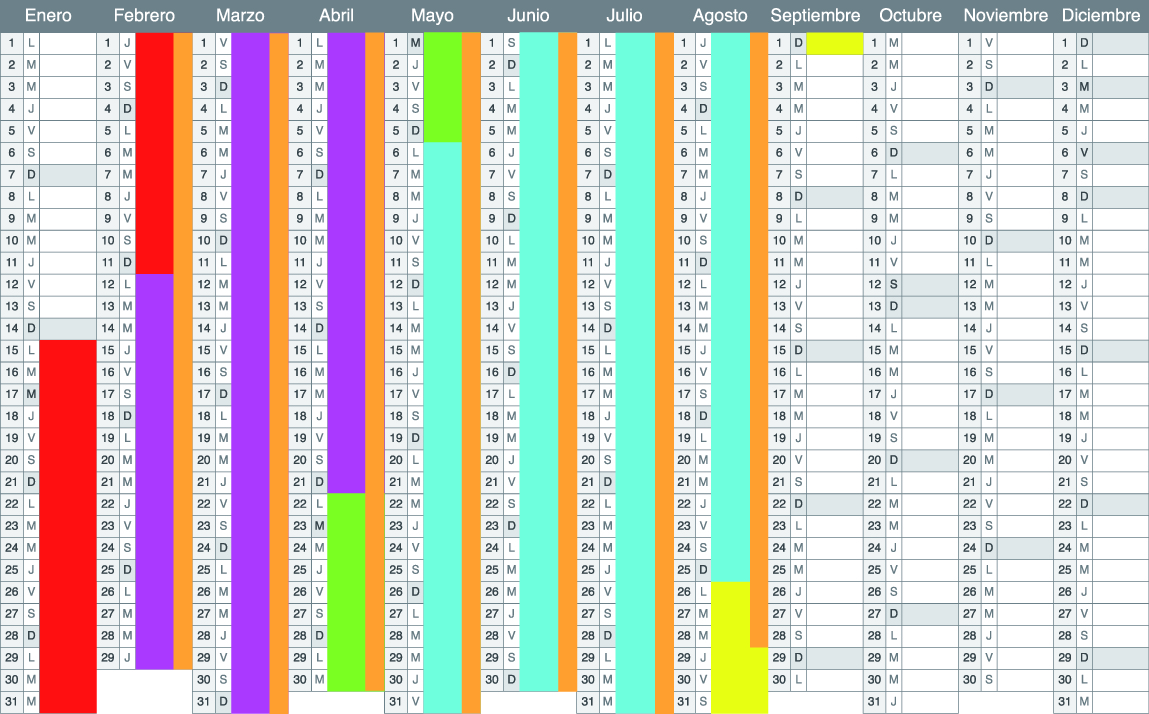
\includegraphics[width=1\textwidth]{imgs/tabla-planning1.jpg}
	\caption{Planificación temporal en el calendario}
	\label{fig:planning1}
\end{figure}

\begin{figure}[H]
	\centering
	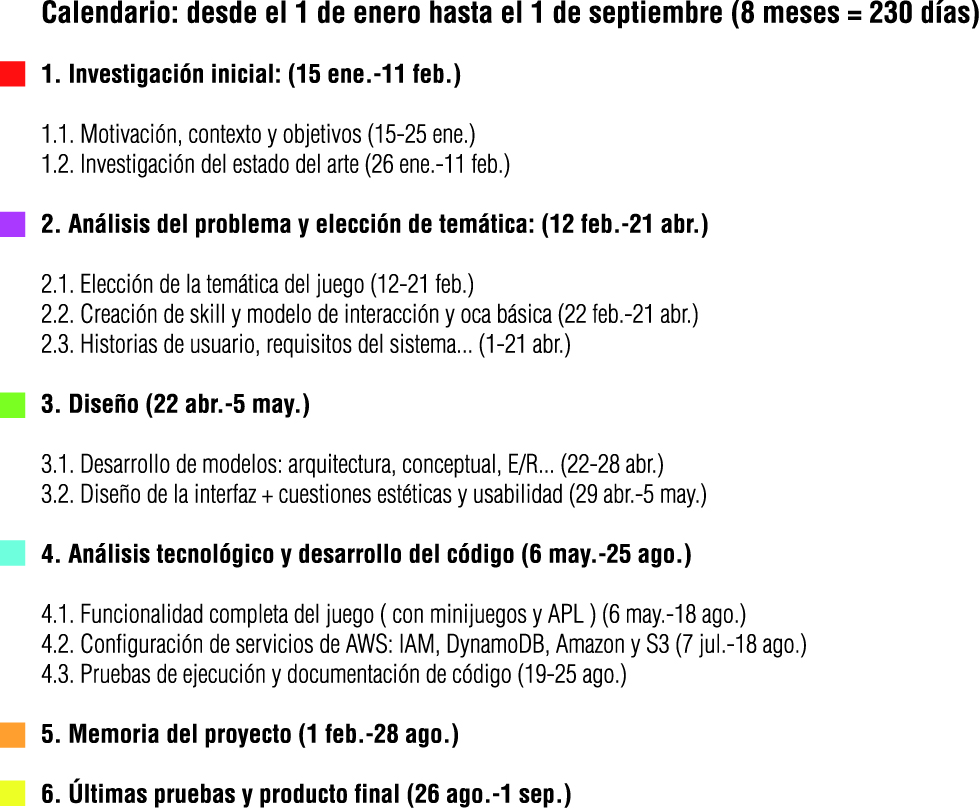
\includegraphics[width=1\textwidth]{imgs/tabla-planning2.jpg}
	\caption{Leyenda de la planificación temporal por (sub)tareas}
	\label{fig:planning2}
\end{figure}

\newpage

\subsection{Metodología}

La metodología describe las técnicas y procesos que se seguirán para desarrollar el proyecto, incluyendo las herramientas y tecnologías utilizadas, los roles y responsabilidades del equipo y los métodos de comunicación y gestión del proyecto. En este caso, se va a emplear la metodología de \textit{desarrollo ágil}.

El método de desarrollo ágil utiliza un enfoque iterativo y flexible, facilitando la adaptación a cambios y la entrega continua de valor al usuario. Esta metodología es especialmente efectiva en entornos donde las necesidades del usuario y el mercado pueden cambiar rápidamente, y donde la colaboración y la comunicación efectiva entre los miembros del equipo y con el cliente son fundamentales para el éxito del proyecto \parencite{metodologiaAgil}.

El desarrollo ágil para una aplicación se divide en varias etapas que se alinean con las prácticas y principios de dicha metodología. Estas fases incluyen:

\begin{enumerate}
    \item \textbf{Análisis del problema}: se centra en comprender las necesidades del usuario y los requisitos del sistema. En el contexto de una aplicación, implica la creación de historias de usuario y casos de uso, que son esenciales para definir las funcionalidades que la aplicación debe ofrecer.
    \item \textbf{Diseño}: se planifican las soluciones técnicas y se definen los detalles de diseño, como la arquitectura de la aplicación, el modelo E/R y el diseño de la interfaz de usuario. El diseño conceptual y los bocetos y mockups de esta fase preparan el camino para la implementación.
    \item \textbf{Desarrollo}: se trabaja para implementar las soluciones diseñadas. Esto incluye la codificación, integración de componentes y configuración del entorno de desarrollo.
    \item \textbf{Pruebas}: su realización permite corregir errores a tiempo. Esto asegura que la aplicación funcione como se espera y cumpla con los requisitos definidos en las etapas anteriores.
    \item \textbf{Despliegue}: una vez que la aplicación ha sido probada y se ha asegurado de que cumple con los requisitos y expectativas, se despliega para su uso.
    \item \textbf{Revisión y mejora continua}: tras el despliegue, se puede incluir la recopilación de comentarios de los usuarios, la identificación de áreas de mejora en el proceso de desarrollo y las implementaciones de cambios para mejorarla en iteraciones futuras.
\end{enumerate}


\subsection{Presupuesto}

El presupuesto es una herramienta clave para gestionar los recursos del proyecto, desde el asignamiento de recursos humanos hasta la adquisición de equipamiento y materiales necesarios. Permite estimar los costos asociados a cada entregable y recurso requerido, estableciendo un cronograma de gastos y asignando responsabilidades para el control de los mismos.

\subsubsection{Recursos humanos}
Incluye las personas involucradas en el proyecto, tanto en las etapas previas al desarrollo como durante el mismo.

\begin{table}[H]
    \centering
    \begin{tabular}{|c|c|}
    \hline
    \rowcolor{lightgray}
    \textbf{Descripción} & \textbf{Coste (€)}\\
    \hline
    Desarrollador(a) de software & 1500 \\
    \hline
    Ingeniero/a de Cloud Computing & 1600 \\
    \hline
    Psicólogo/a & 200 \\
    \hline
    Expertos en Gerontología de la UGR & Colaboración voluntaria \\
    \hline
    \end{tabular}
    \caption{Presupuesto para recursos humanos}
    \label{tab:presupuesto-personal}
\end{table}

\subsubsection{Hardware}
Todos los dispositivos físicos y electrónicos necesarios para llevar a cabo la aplicación.

\begin{table}[H]
    \centering
    \begin{tabular}{|c|c|}
    \hline
    \rowcolor{lightgray}
    \textbf{Descripción} & \textbf{Coste (€)}\\
    \hline
    HP 15s Intel Core i5-1035G1/16GB/1TB/15.6" & 550-650 \\
    \hline
    Alexa Echo Show & 70 \\
    \hline
    \end{tabular}
    \caption{Presupuesto para hardware}
    \label{tab:presupuesto-hw}
\end{table}

\subsubsection{Software}
Los programas utilizados durante todo el proceso, desde el análisis y diseño hasta el desarrollo y despliegue.  

\begin{table}[H]
    \centering
    \begin{tabular}{|c|c|}
    \hline
    \rowcolor{lightgray}
    \textbf{Descripción} & \textbf{Coste (€)}\\
    \hline
    Visual Paradigm & Licencia académica gratuita \\
    \hline
    Amazon Web Services (AWS) & 10 \\
    \hline
    TeXstudio & 0 \\
    \hline
    Visual Studio Code & 0 \\
    \hline
    GitHub & 0 \\
    \hline
    Alexa Developer Console & 0 \\
    \hline
    \end{tabular}
    \caption{Presupuesto para software}
    \label{tab:presupuesto-sw}
\end{table}

\subsubsection{Resumen de presupuesto}
Al combinar la cantidad total de presupuesto de recursos humanos, hardware y software, se elabora la siguiente tabla:

\begin{table}[H]
    \centering
    \begin{tabular}{|c|c|}
        \hline
        \rowcolor{lightgray}
        \textbf{Descripción} & \textbf{Coste (€)} \\
        \hline
        Recursos humanos & 3100 \\
        \hline
        Hardware & 670 \\
        \hline
        Software & 10 \\
        \hline
        \textbf{Total} & \textbf{3780} \\
        \hline
    \end{tabular}
    \caption{Tabla general de presupuestos}
    \label{tab:presupuesto-total}
\end{table}
